\baselineskip=8mm
% \renewcommand{\thesubsection}{\thechapter.\arabic{subsection}}
\numberwithin{equation}{chapter}
\numberwithin{equation}{section}
\renewcommand{\thesubsection}{\arabic{subsection}.}
\renewcommand{\theequation}{\thesection.\arabic{equation}}
\renewcommand{\thesection}{}
\renewcommand{\thesubsubsection}{\thesubsection\arabic{subsubsection}.}



\section{Entity-Relationship Diagram}
\begin{figure}[h]
    \centering
    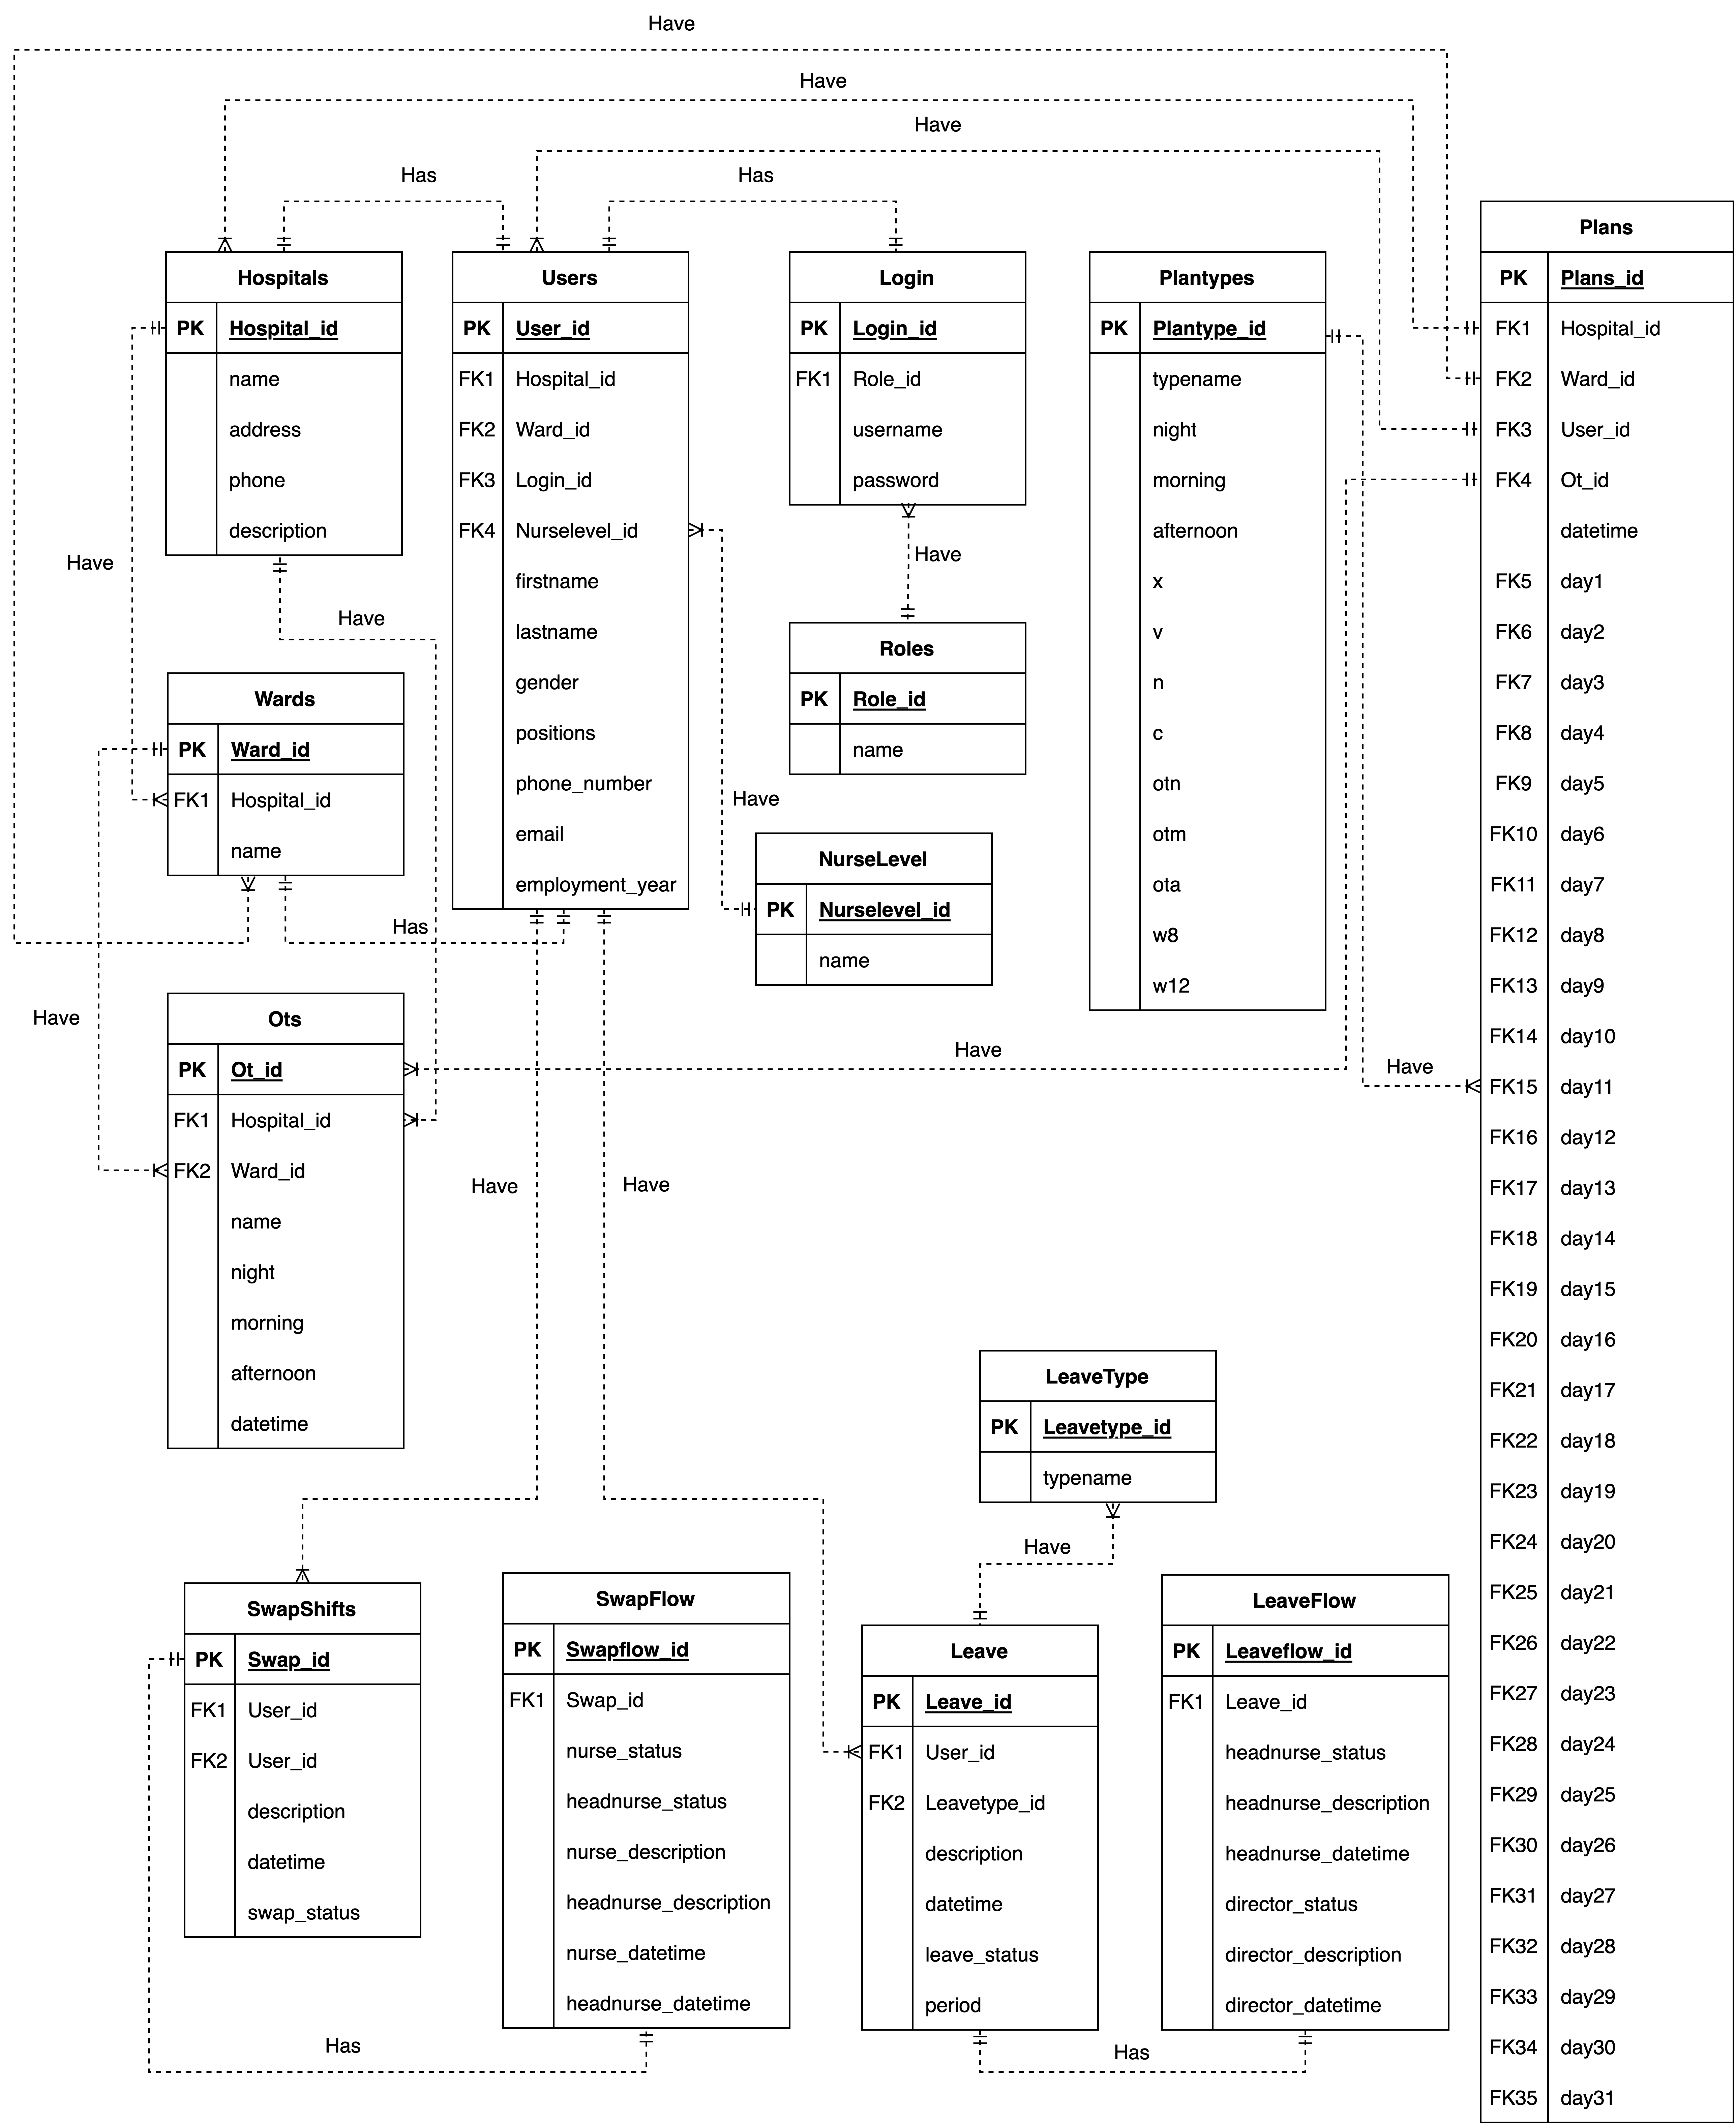
\includegraphics[width=0.9\textwidth]{ER Diagram.png}
    \caption{Entity-Relationship Diagram}
    \end{figure}

\clearpage

\section{Data Dictionary}

\vspace{1cm}


\begin{table}[h]
    \captionsetup{justification=raggedright,singlelinecheck=false}
    \centering
    \fontsize{8}{10}\selectfont	
    \resizebox{\textwidth}{!}{%
    \begin{tabular}{lccccc}
        \toprule
        \multicolumn{6}{c}{Hospitals} \\ \hline
        Name & Datatype & Length & Description & Example & Key \\ \hline
        Hospital\_id & int & 5  & รหัสโรงพยาบาล  & 00001 & PK \\
        name& char & 50 & ชื่อโรงพยาบาล & University Of Phayao Hospital &  \\
        address& Char  & 60 &  ที่อยู่โรงพยาบาล & ต.แม่กา อ.เมืองพะเยา จ.พะเยา &  \\
        phone& Char  & 10 & เบอร์โทรศัพท์ & 054466758 & \\
        description& Char & 100& ราบละเอียดของโรงพยาบาล & uph.up.ac.th & \\
        \bottomrule
    \end{tabular}%
    }
    \caption{Data Dictionary ของตาราง Hospitals}
\end{table}


\begin{table}[h]
    \captionsetup{justification=raggedright,singlelinecheck=false}
    \centering
    \fontsize{8}{10}\selectfont	
    \resizebox{\textwidth}{!}{%
    \begin{tabular}{lccccc}
        \toprule
        \multicolumn{6}{c}{Wards} \\ \hline
        Name & Datatype & Length & Description & Example & Key \\ \hline
        Ward\_id & int & 2  & รหัสวอร์ด  & 01 & PK \\
        Hospital\_id & int & 5  & รหัสโรงพยาบาล  & 00001 & FK \\
        name& char & 50 & ชื่อวอร์ด & การพยาบาลผู้ป่วยใน &  \\
        \bottomrule
    \end{tabular}%
    }
    \caption{Data Dictionary ของตาราง Wards}
\end{table}

\begin{table}[h]
    \captionsetup{justification=raggedright,singlelinecheck=false}
    \centering
    \fontsize{8}{10}\selectfont	
    \resizebox{\textwidth}{!}{%
    \begin{tabular}{lccccc}
        \toprule
        \multicolumn{6}{c}{Login} \\ \hline
        Name & Datatype & Length & Description & Example & Key \\ \hline
        Role\_id & int & 2  & รหัสสิทธิ์การใช้งาน  & 01 & FK \\
        name& char & 50 & ชื่อสิทธิ์การใช้งาน & ผู้ดูแลระบบ &  \\
        \bottomrule
    \end{tabular}%
    }
    \caption{Data Dictionary ของตาราง Role}
\end{table}

\begin{table}[h]
    \captionsetup{justification=raggedright,singlelinecheck=false}
    \centering
    \fontsize{8}{10}\selectfont	
    \resizebox{\textwidth}{!}{%
    \begin{tabular}{lccccc}
        \toprule
        \multicolumn{6}{c}{Login} \\ \hline
        Name & Datatype & Length & Description & Example & Key \\ \hline
        Login\_id & int & 5  & รหัสการเข้าสู่ระบบ  & 00001 & PK \\
        Role\_id & int & 2  & รหัสสิทธิ์การใช้งาน  & 01 & FK \\
        username& char & 30 & ชื่อผู้ใช้ & Sirawittop &  \\
        password& char & 30 & รหัสผ่าน & ZXhhbXBsZQ== &  \\
        \bottomrule
    \end{tabular}%
    }
    \caption{Data Dictionary ของตาราง Login}
\end{table}


\begin{table}[h]
    \captionsetup{justification=raggedright,singlelinecheck=false}
    \centering
    \fontsize{8}{10}\selectfont	
    \resizebox{\textwidth}{!}{%
    \begin{tabular}{lccccc}
        \toprule
        \multicolumn{6}{c}{Ots} \\ \hline
        Name & Datatype & Length & Description & Example & Key \\ \hline
        Ot\_id & int & 5  & รหัสการเข้าสู่ระบบ  & 00001 & PK \\
        Hospital\_id & int & 5  & รหัสโรงพยาบาล  & 00001 & FK \\
        Ward\_id & int & 2  & รหัสวอร์ด  & 01 & FK \\
        name& char & 20 & ชื่อตำแหน่งของพยาบาล & หัวหน้าพยาบาล &  \\
        night & int & 2 & จำนวนเวรกลางคืน & 2 &  \\
        morning & int & 2 & จำนวนเวรกลางวัน & 2 &  \\
        afternoon & int & 2 & จำนวนเวรกลางค่ำ & 2 &  \\
        datetime & datetime &  & วันที่และเวลา & 2022-12-12 12:12:12 &  \\


        \bottomrule
    \end{tabular}%
    }
    \caption{Data Dictionary ของตาราง Ots}
\end{table}

\begin{table}[h]
    \captionsetup{justification=raggedright,singlelinecheck=false}
    \centering
    \fontsize{8}{10}\selectfont	
    \resizebox{\textwidth}{!}{%
    \begin{tabular}{lccccc}
        \toprule
        \multicolumn{6}{c}{SwapShifts} \\ \hline
        Name & Datatype & Length & Description & Example & Key \\ \hline
        Swap\_id & int & 5  & รหัสการแลกเวร  & 00001 & PK \\
        User\_id & int & 5  & รหัสผู้ใช้งาน  & 00001 & FK \\
        User\_id2 & int & 5  & รหัสผู้ใช้งาน  & 00002 & FK \\
        description & char & 100 & รายละเอียดการแลกเวร & พาลูกไปแข่งขัน &  \\ 
        datetime & datetime &  & วันที่และเวลา & 2022-12-12 12:12:12 &  \\
        swap\_status & char & 10 & สถานะการแลกเวร & รอการอนุมัติ &  \\


        \bottomrule
    \end{tabular}%
    }
    \caption{Data Dictionary ของตาราง SwapShifts}
\end{table}

\begin{table}[h]
    \captionsetup{justification=raggedright,singlelinecheck=false}
    \centering
    \fontsize{8}{10}\selectfont	
    \resizebox{\textwidth}{!}{%
    \begin{tabular}{lccccc}
        \toprule
        \multicolumn{6}{c}{SwapFlow} \\ \hline
        Name & Datatype & Length & Description & Example & Key \\ \hline
        Swapflow\_id & int & 5  & รหัสความคืบหน้าการแลกเวร  & 00001 & PK \\
        Swap\_id & int & 5  & รหัสการแลกเวร  & 00001 & FK \\
        nurse\_status & char & 10 & สถานะการแลกเวรของพยาบาล & รอการอนุมัติ &  \\
        headnurse\_status & char & 10 & สถานะการแลกเวรของหัวหน้าพยาบาล & รอการอนุมัติ &  \\
        nurse\_description & char & 100 & คำอธิบายการยืนยันของพยาบาล & ไม่สะดวกในวันนี้ &  \\
        headnurse\_description & char & 100 & คำอธิบายการยืนยันของหัวหน้าพยาบาล & จำนวนพยาบาลที่มีประสบการณ์ไม่พอ &  \\
        nurse\_datetime & datetime &  & วันที่และเวลาของพยาบาลที่ยืนยัน & 2022-12-12 12:12:12 &  \\
        headnurse\_datetime & datetime &  & วันที่และเวลาของหัวหน้าพยาบาลที่ยืนยัน & 2022-12-12 12:12:12 &  \\

        \bottomrule
    \end{tabular}%
    }
    \caption{Data Dictionary ของตาราง SwapFlow}
\end{table}


\begin{table}[h]
    \captionsetup{justification=raggedright,singlelinecheck=false}
    \centering
    \fontsize{8}{10}\selectfont	
    \resizebox{\textwidth}{!}{%
    \begin{tabular}{lccccc}
        \toprule
        \multicolumn{6}{c}{Leave} \\ \hline
        Name & Datatype & Length & Description & Example & Key \\ \hline
        Leave\_id & int & 5  & รหัสการลา  & 00001 & PK \\
        User\_id & int & 5  & รหัสผู้ใช้งาน  & 00001 & FK \\
        description & char & 100 & รายละเอียดการลา & ไปงานศพ &  \\
        datetime & datetime &  & วันที่และเวลา & 2022-12-12 12:12:12 &  \\
        leave\_status & char & 10 & สถานะการลา & รอการอนุมัติ &  \\
        period & char & 10 & ช่วงเวลาการลา & ลาป่วย &  \\

        \bottomrule
    \end{tabular}%
    }
    \caption{Data Dictionary ของตาราง Leave}
\end{table}


\begin{table}[h]
    \captionsetup{justification=raggedright,singlelinecheck=false}
    \centering
    \fontsize{8}{10}\selectfont	
    \resizebox{\textwidth}{!}{%
    \begin{tabular}{lccccc}
        \toprule
        \multicolumn{6}{c}{LeaveFlow} \\ \hline
        Name & Datatype & Length & Description & Example & Key \\ \hline
        Leaveflow\_id & int & 5  & รหัสความคืบหน้าการลา  & 00001 & PK \\
        Leave\_id & int & 5  & รหัสการลา  & 00001 & FK \\
        headnurse\_status & char & 10 & สถานะการยืนยันของหัวหน้าพยาบาล & รอการอนุมัติ &  \\   
        headnurse\_description & char & 100 & คำอธิบายการยืนยันของหัวหน้าพยาบาล & จำนวนพยาบาลที่มีประสบการณ์ไม่พอ &  \\
        headnurse\_datetime & datetime &  & วันที่และเวลาของหัวหน้าพยาบาลที่ยืนยัน & 2022-12-12 12:12:12 &  \\
        director\_status     & char & 10 & สถานะการยืนยันของผู้อำนวยการ & รอการอนุมัติ &  \\
        director\_description & char & 100 & คำอธิบายการยืนยันของผู้อำนวยการ & ไม่สามารถลาได้เพราะลาบ่อย &  \\
        director\_datetime    & datetime &  & วันที่และเวลาของผู้อำนวยการที่ยืนยัน & 2022-12-12 12:12:12 &  \\


        \bottomrule
    \end{tabular}%
    }
    \caption{Data Dictionary ของตาราง LeaveFlow}
\end{table}


\begin{table}[h]
    \captionsetup{justification=raggedright,singlelinecheck=false}
    \centering
    \fontsize{8}{10}\selectfont	
    \resizebox{\textwidth}{!}{%
    \begin{tabular}{lccccc}
        \toprule
        \multicolumn{6}{c}{Users} \\ \hline
        Name & Datatype & Length & Description & Example & Key \\ \hline
        User\_id & int & 5  & รหัสผู้ใช้งาน  & 00001 & PK \\
        Hospital\_id & int & 5  & รหัสโรงพยาบาล  & 00001 & FK \\
        Ward\_id & int & 2  & รหัสวอร์ด  & 01 & FK \\
        Login\_id & int & 5  & รหัสการเข้าสู่ระบบ  & 00001 & FK \\
        Nurselevel\_id & int & 2  & รหัสระดับของพยาบาล  & 01 & FK \\  
        firstname & char & 30 & ชื่อ & Sirawit &  \\
        lastname & char & 30 & นามสกุล & Opas &  \\
        gender & char & 10 & เพศ & ชาย &  \\
        position & char & 30 & ตำแหน่ง & พยาบาล &  \\
        phone\_number & char & 10 & เบอร์โทรศัพท์ & 0987654321 &  \\
        email & char & 50 & อีเมล & sirawit.code@gmail.com & \\
        employment\_year & int & 4 & ปีการทำงาน & 5 &  \\            
        \bottomrule
    \end{tabular}%
    }
    \caption{Data Dictionary ของตาราง Users}
\end{table}


\begin{table}[h]
    \captionsetup{justification=raggedright,singlelinecheck=false}
    \centering
    \fontsize{8}{10}\selectfont	
    \resizebox{\textwidth}{!}{%
    \begin{tabular}{lccccc}
        \toprule
        \multicolumn{6}{c}{LeaveType} \\ \hline
        Name & Datatype & Length & Description & Example & Key \\ \hline
        LeaveType\_id & int & 5  & รหัสประเภทการลา  & 00001 & PK \\
        typename & char & 30 & ชื่อประเภทการลา & ลาป่วย &  \\
        \bottomrule
    \end{tabular}%
    }
    \caption{Data Dictionary ของตาราง LeaveType}
\end{table}

\begin{table}[h]
    \captionsetup{justification=raggedright,singlelinecheck=false}
    \centering
    \fontsize{8}{10}\selectfont	
    \resizebox{\textwidth}{!}{%
    \begin{tabular}{lccccc}
        \toprule
        \multicolumn{6}{c}{NurseLevel} \\ \hline
        Name & Datatype & Length & Description & Example & Key \\ \hline
        Nurselevel\_id & int & 2  & รหัสระดับของพยาบาล  & 01 & PK \\
        name & char & 30 & ชื่อระดับของพยาบาล & พยาบาลปฏิบัติการ &  \\
        \bottomrule
    \end{tabular}%
    }
    \caption{Data Dictionary ของตาราง NurseLevel}
\end{table}


\begin{table}[h]
    \captionsetup{justification=raggedright,singlelinecheck=false}
    \centering
    \fontsize{8}{10}\selectfont	
    \resizebox{\textwidth}{!}{%
    \begin{tabular}{lccccc}
        \toprule
        \multicolumn{6}{c}{Plantypes} \\ \hline
        Name & Datatype & Length & Description & Example & Key \\ \hline
        Plantypes\_id & int & 2  & รหัสแผนการทำงาน  & 01 & PK \\
        typename & char & 30 & ชื่อแผนการทำงาน & ลาป่าย &  \\
        night & boolean & 2 & เวรดึก & 1 &  \\
        morning & boolean & 2 & เวรเช้า & 1 &  \\
        afternoon & boolean & 2 & เวรบ่าย & 1 &  \\
        x & boolean & 2 & เวรหยุด & 0 &  \\
        v & boolean & 2 & ลาพักผ่อน & 1 &  \\
        n & boolean & 2 & นอกเวลา & 1 &  \\
        c & boolean & 2 & on call duty & 1 &  \\
        otn & boolean & 2 & การทำงานนอกเวลาดึก & 1 &  \\
        otm & boolean & 2 & การทำงานนอกเวลาเช้า & 0 &  \\
        ota & boolean & 2 & การทำงานนอกเวลาบ่าย & 0 &  \\
        w8 & boolean & 2 & ทำงานแบบ 8 ชั่วโมง & 0 &  \\
        w12 & boolean & 2 & ทำงานแบบ 12 ชั่วโมง & 1 &  \\
        \bottomrule
    \end{tabular}%
    }
    \caption{Data Dictionary ของตาราง Plantypes}
\end{table}


\begin{table}[h]
    \captionsetup{justification=raggedright,singlelinecheck=false}
    \centering
    \fontsize{8}{10}\selectfont	
    \resizebox{\textwidth}{!}{%
    \begin{tabular}{lccccc}
        \toprule
        \multicolumn{6}{c}{Plans} \\ \hline
        Name & Datatype & Length & Description & Example & Key \\ \hline
        Plans\_id & int & 5  & รหัสแผนการทำงาน  & 00001 & PK \\
        Hospital\_id & int & 5  & รหัสโรงพยาบาล  & 00001 & FK \\
        Ward\_id & int & 2  & รหัสวอร์ด  & 01 & FK \\
        User\_id & int & 5  & รหัสผู้ใช้งาน  & 00001 & FK \\
        Ots\_id & int & 5  & รหัสการทำงานนอกเวลา  & 00001 & FK \\
        datetime & datetime &  & วันที่และเวลา & 2022-12-12 12:12:12 &  \\
        day1 & int & 3 & วันที่1  & 1 &  \\
        day2 & int & 3 & วันที่2  & 4 &  \\
        ... & ... & ... & ... & ... &  \\
        day31 & int & 3 & วันที่31  & 6 &  \\


        \bottomrule
    \end{tabular}%
    }
    \caption{Data Dictionary ของตาราง Plans}
\end{table}